\documentclass[conference, onecolumn]{IEEEtran} % Replace onecolumn with twocolumn if needed
% Report template for Mälardalen University
% Original template can be found: 
% https://www.overleaf.com/latex/templates/ieee-bare-demo-template-for-conferences/ypypvwjmvtdf
% Template file structure organised by: Emil Persson
% The following packages should follow the IEEE conference guidelines.

% Swedish language package 
\usepackage[utf8]{inputenc}
\usepackage[T1]{fontenc}
\usepackage[swedish,english]{babel}

% Graphics
\usepackage{graphicx, float, subfigure, blindtext}

\newcommand\IEEEhyperrefsetup{
bookmarks=true,bookmarksnumbered=true,%
colorlinks=true,linkcolor={black},citecolor={black},urlcolor={black}%
}

% Preferred hyperref setup, Michael Shell
\usepackage[\IEEEhyperrefsetup, pdftex]{hyperref}

% Maths
\usepackage{mathtools}

% These packages must be at the end
\usepackage[nolist,nohyperlinks]{acronym}
\usepackage{cleveref}
\graphicspath{{images/}}
% \acrodef{acronym}[short name]{full name}
\acrodef{IC}[IC]{Integrated Circuit}
% \acrodef{svm}[SVM]{Support Vector Machine}
\newacro{svm}[SVM]{Support Vector Machine}
% Example use \ac{IC} for printing "Integrated Circuit (IC), use \ac{IC} again and it will print (IC)"
% For plural use \acp{IC} for short and \aclp{IC} for long.
% For more see: http://ftp.acc.umu.se/mirror/CTAN/macros/latex/contrib/acronym/acronym.pdf

% Swedish language package 
\usepackage[utf8]{inputenc}
\usepackage[T1]{fontenc}
\usepackage[swedish,english]{babel}

% Graphics
\usepackage{graphicx, float, subfigure, blindtext}

% \newcommand\IEEEhyperrefsetup{
% bookmarks=true,bookmarksnumbered=true,%
% colorlinks=true,linkcolor={black},citecolor={black},urlcolor={black}%
% }

% Preferred hyperref setup, Michael Shell
% \usepackage[\IEEEhyperrefsetup, pdftex]{hyperref}

% Maths
\usepackage{mathtools}
\usepackage{multirow}
\usepackage{listings}
% These packages must be at the end
\usepackage[nolist,nohyperlinks]{acronym}
\usepackage{cleveref}
\graphicspath{{images/}}

% Remove section first paragraph indent
\usepackage{titlesec}
\titlespacing*{\section}{0pt}{*1}{*1}
\titlespacing*{\subsection}{0pt}{*1}{*1}
\renewcommand{\thesubsubsection}{\arabic{subsubsection}}
\titleformat{\subsubsection}[runin]{\itshape}{\thesubsubsection)}{1em}{}[:]
\titlespacing*{\subsubsection}{\parindent}{0pt}{*1}

% Include authors
\author{\IEEEauthorblockN{
Carl-Johan Höglind\IEEEauthorrefmark{1},
Author 2\IEEEauthorrefmark{2}
}

\IEEEauthorblockA{
School of Innovation, Design and Engineering\\
Mälardalen University, Västerås, Sweden\\
Email:
\IEEEauthorrefmark{1}chd16002@student.mdu.se,
\IEEEauthorrefmark{2}author2@student.mdu.se
}}

% The report title.
\title{Assignment 2, Embedded Systems II\\
Mälardalen University}

% Document begins here
\begin{document}

    % Create the title.
    \maketitle
    % Example sections, name them according to specific needs.
    \section{Question 1} 

    \section{Question 2}
        \subsection{a}
            Sufficient schedulability test for RM scheduling: $U <= n(2^{1/n} - 1)$ \\ where n is the number of tasks in the task set and U is the processor utilization factor, $U = \sum_{i=1}^{n} \frac{C_i}{T_i}$. 

        \renewcommand{\arraystretch}{1.4}
        \begin{figure}[H]
        \centering
        \begin{minipage}{0.5\textwidth}
            \begin{table}[H]
            \centering
            \begin{tabular}{|l|l|l|}
                \hline
                \textbf{Task}   & \textbf{T=D}  & \textbf{C}  \\ \hline
                A               & 3             & 1           \\ \hline
                B               & 5             & 2           \\ \hline
                C               & 2             & 0.5         \\ \hline

            \end{tabular}
            \end{table}
        \end{minipage}%
        \caption{Task set}
        \label{fig:Taskset}
        \end{figure}
    \renewcommand{\arraystretch}{1.0}

        \subsubsection{Task set schedulable?}
        $U = \sum_{i=1}^{n} \frac{C_i}{T_i} = \frac{1}{3} + \frac{2}{5} + \frac{0.5}{2} = 0.98$ \\
        $U <= n(2^{1/n} - 1) = 3(2^{1/3} - 1) = 0.78$ \\
        Since the statement $U <= n(2^{1/n} - 1)$ is false in this case, the task set cannot be proven to be schedulable with this sufficient test method.

        \subsection{b}
            \subsubsection{Exact schedulability test, Tracing}
            \begin{figure}[H]
                \centering
                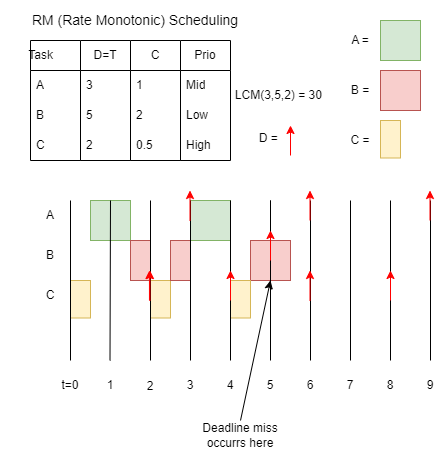
\includegraphics[width=0.5\textwidth]{images/Ass1Q2.drawio.png}
                \caption{Tracing of the task set proves that it is not schedulable with RM.}
                \label{fig:tracing}
            \end{figure}

            As demonstrated in figure \ref{fig:Taskset}, the task set is not schedulable with RM scheduling. The task set is not schedulable because task B misses its deadline at $t = 5$.

    \appendix
\section{First Appendix}

The code written in FpsCalc:
\begin{lstlisting}
	! =======================================================================
	! ============================ Emil Broberg =============================
	! =======================================================================
	
	! Global variables declarations
	scalar
		LoadNode_A, LoadNode_B, LoadNode_C, LoadNode_D, LoadNode_CAN;
	scalar
		MBS_S_senseA, MBS_S_senseB, MBS_S_senseC, MBS_S_actA, MBS_S_actB, MBS_S_actC;
	scalar
		Trans_t_S_senseA, Trans_t_S_senseB, Trans_t_S_senseC, Trans_t_S_actA, 
		Trans_t_S_actB, Trans_t_S_actC;
	indexed
		Jafter1, Jafter2, Jafter3, Jafter4, TransactionsR;
	tasks
		Trans1, Trans2, Trans3;
	
	! =======================================================================
	
	system Node_A {
		declarations {
			indexed T, D, C, W, J, R, LoadArray;
			priority P;
			scalar B;
	
			! Tasks in Node A
			tasks Sense_A, Act_A, P1A, P2A, P3A;
		}
	
		initialise {
			! Period for each task
			T[Sense_A] = 10;
			T[Act_A] = 10;
			T[P1A] = 5;
			T[P2A] = 15;
			T[P3A] = 50;
	
			! Release Jitter for each task
			J[Sense_A] = 0;
			J[Act_A] = 0;
			J[P1A] = 0;
			J[P2A] = 2;
			J[P3A] = 5;
	
			! Execution time for each task
			C[Sense_A] = 1;
			C[Act_A] = 1;
			C[P1A] = 1;
			C[P2A] = 2;
			C[P3A] = 1;
	
			! Priority according to Rate Monotonic, 1 = Highest priority
			P[Sense_A] = 2;
			P[Act_A] = 3;
			P[P1A] = 1;
			P[P2A] = 4;
			P[P3A] = 5;
	
			! Deadline for each task
			D[Sense_A] = 15;
			D[Act_A] = 15;
			D[P1A] = 2;
			D[P2A] = 10;
			D[P3A] = 25;
	
			! Blocking is zero since we use no semaphores and RM-scheduling
			B = 0;
		}
	
		formulas {
			! Act_A inherits Jitter from previously executed tasks
			J[Act_A] = Jafter4[Trans1];
	
			! Calculate window of interference
			W[i] = C[i] + B + sigma(hp, ceiling((W[i]+J[j])/T[j]) * C[j]);
			! Calculate the response-time
			R[i] = W[i] + J[i];
			
			! Jitter to be inherited by Node_CAN
			Jafter1[Trans1] = R[Sense_A];
	
			! Save R in global array TransactionsR
			TransactionsR[Trans1] = R[Act_A];
	
			! Load (utilization)
			LoadArray[i] = C[i] / T[i];
			! Convert to percent to display as result
			LoadNode_A = 100 * (LoadArray[Sense_A] + LoadArray[Act_A] 
			+ LoadArray[P1A] + LoadArray[P2A] + LoadArray[P3A]);
		}
	}
	
	! =======================================================================
	
	system Node_B {
		declarations {
			indexed T, D, C, W, J, R, LoadArray;
			priority P;
			scalar B;
	
			! Tasks in Node B
			tasks Sense_B, Act_B, P1B, P2B, P3B;
		}
	
		initialise {
			! Period for each task
			T[Sense_B] = 10;
			T[Act_B] = 10;
			T[P1B] = 5;
			T[P2B] = 15;
			T[P3B] = 50;
	
			! Release Jitter for each task
			J[Sense_B] = 0;
			J[Act_B] = 0;
			J[P1B] = 0;
			J[P2B] = 2;
			J[P3B] = 5;
	
			! Execution time for each task
			C[Sense_B] = 1;
			C[Act_B] = 1;
			C[P1B] = 1;
			C[P2B] = 2;
			C[P3B] = 1;
	
			! Priority according to Rate Monotonic, 1 = Highest priority
			P[Sense_B] = 2;
			P[Act_B] = 3;
			P[P1B] = 1;
			P[P2B] = 4;
			P[P3B] = 5;
	
			! Deadline for each task
			D[Sense_B] = 20;
			D[Act_B] = 20;
			D[P1B] = 2;
			D[P2B] = 10;
			D[P3B] = 25;
	
			! Blocking is zero since we use no semaphores and RM-scheduling
			B = 0;
		}
	
		formulas {
			! Act_B inherits Jitter from previously executed tasks
			J[Act_B] = Jafter4[Trans2];
	
			! Calculate window of interference
			W[i] = C[i] + B + sigma(hp, ceiling((W[i]+J[j])/T[j]) * C[j]);
			! Calculate the response-time
			R[i] = W[i] + J[i];
			
			! Jitter to be inherited by Node_CAN
			Jafter1[Trans2] = R[Sense_B];
	
			! Save R in global array TransactionsR
			TransactionsR[Trans2] = R[Act_B];
	
			! Load (utilization)
			LoadArray[i] = C[i] / T[i];
			! Convert to percent to display as result
			LoadNode_B = 100 * (LoadArray[Sense_B] + LoadArray[Act_B] 
			+ LoadArray[P1B] + LoadArray[P2B] + LoadArray[P3B]);
		}
	}
	
	! =======================================================================
	
	system Node_C {
		declarations {
			indexed T, D, C, W, J, R, LoadArray;
			priority P;
			scalar B;
	
			! Tasks in Node C
			tasks Sense_C, Act_C, P1C, P2C, P3C;
		}
	
		initialise {
			! Period for each task
			T[Sense_C] = 20;
			T[Act_C] = 20;
			T[P1C] = 5;
			T[P2C] = 15;
			T[P3C] = 50;
	
			! Release Jitter for each task
			J[Sense_C] = 0;
			J[Act_C] = 0;
			J[P1C] = 0;
			J[P2C] = 2;
			J[P3C] = 5;
	
			! Execution time for each task
			C[Sense_C] = 2;
			C[Act_C] = 1;
			C[P1C] = 1;
			C[P2C] = 2;
			C[P3C] = 1;
	
			! Priority according to Rate Monotonic, 1 = Highest priority
			P[Sense_C] = 3;
			P[Act_C] = 4;
			P[P1C] = 1;
			P[P2C] = 2;
			P[P3C] = 5;
	
			! Deadline for each task
			D[Sense_C] = 40;
			D[Act_C] = 40;
			D[P1C] = 2;
			D[P2C] = 10;
			D[P3C] = 25;
	
			! Blocking is zero since we use no semaphores and RM-scheduling
			B = 0;
		}
	
		formulas {
			! Act_C inherits Jitter from previously executed tasks
			J[Act_C] = Jafter4[Trans3];
	
			! Calculate window of interference
			W[i] = C[i] + B + sigma(hp, ceiling((W[i]+J[j])/T[j]) * C[j]);
			! Calculate the response-time
			R[i] = W[i] + J[i];
			
			! Jitter to be inherited by Node_CAN
			Jafter1[Trans3] = R[Sense_C];
	
			! Save R in global array TransactionsR
			TransactionsR[Trans3] = R[Act_C];
	
			! Load Utilization
			LoadArray[i] = C[i] / T[i];
			! Convert to percent to display as result
			LoadNode_C = 100 * (LoadArray[Sense_C] + LoadArray[Act_C] 
			+ LoadArray[P1C] + LoadArray[P2C] + LoadArray[P3C]);
		}
	}
	
	! =======================================================================
	
	system Node_D{
		declarations {
			indexed T, J, C, W, R, LoadArray;
			priority P;
			scalar B;
	
			! Tasks in Node D
			tasks CalcA, CalcB, CalcC;
		}
	
		initialise {
			! Period for each task
			T[CalcA] = 10;
			T[CalcB] = 10;
			T[CalcC] = 20;
	
			! Release Jitter for each task
			J[CalcA] = 0;
			J[CalcB] = 0;
			J[CalcC] = 0;
	
			! Execution time for each task
			C[CalcA] = 1;
			C[CalcB] = 2;
			C[CalcC] = 4;
	
			! Priority according to Rate Monotonic, 1 = Highest priority
			P[CalcA] = 1;
			P[CalcB] = 2;
			P[CalcC] = 3;
	
			! Blocking is zero since we use no semaphores and RM-scheduling
			B = 0;
		}
	
		formulas {
			! Jitter inherited from previous tasks
			J[CalcA] = Jafter2[Trans1];
			J[CalcB] = Jafter2[Trans2];
			J[CalcC] = Jafter2[Trans3];
	
			! Calculate window of interference
			W[i] = C[i] + B + sigma(hp, ceiling((W[i]+J[j])/T[j]) * C[j]);
			! Calculate the response-time
			R[i] = W[i] + J[i];
			
			! Store response-time as jitter to be inherited in the next 
			step of transaction
			Jafter3[Trans1] = R[CalcA];
			Jafter3[Trans2] = R[CalcB];
			Jafter3[Trans3] = R[CalcC];
	
			! Load (utilization)
			LoadArray[i] = C[i] / T[i];
			! Convert to percent to display as result
			LoadNode_D = 100 * (LoadArray[CalcA] + LoadArray[CalcB] 
			+ LoadArray[CalcC]);
		}
	}
	
	! =======================================================================
	
	system Node_CAN {
		declarations {
			indexed S, R, W, T, J, C, MaxBitSize, LoadArray;
			scalar bps, tau, B;
			priority P;
	
			! "Tasks" in CANBUS
			tasks S_senseA, S_actA, S_senseB, S_actB, S_senseC, S_actC;
			
		}
	
		initialise {
			! Data size for all messages (bytes)
			S[S_senseA] = 2;
			S[S_actA] = 1;
			S[S_senseB] = 4;
			S[S_actB] = 2;
			S[S_senseC] = 4;
			S[S_actC] = 4;
	
			! Period of the messages
			T[S_senseA] = 10;
			T[S_actA] = 10;
			T[S_senseB] = 10;
			T[S_actB] = 10;
			T[S_senseC] = 20;
			T[S_actC] = 20;
	
			! Priority of messages, 1 = Highest priority
			P[S_senseA] = 1;
			P[S_actA] = 2;
			P[S_senseB] = 3;
			P[S_actB] = 4;
			P[S_senseC] = 5;
			P[S_actC] = 6;
	
			! Blocking is zero according to assignment description (zero 
			blocking from lower priority messages)
			B = 0;
	
			! CAN transmission speed (bits per second)
			bps = 75000; ! 75kps
		}
	
		formulas {
			! tau is how how many milliseconds it takes to send one bit
			tau = 1/(bps/1000);
	
			! Jitter to be inherited by CAN-BUS from node A, B and C
			J[S_senseA] = Jafter1[Trans1];
			J[S_senseB] = Jafter1[Trans2];
			J[S_senseC] = Jafter1[Trans3];
	
			! Jitter inherited from node D
			J[S_actA] = Jafter3[Trans1];
			J[S_actB] = Jafter3[Trans2];
			J[S_actC] = Jafter3[Trans3];
	
			! MaxBitSize, including stuff-bits (fromula from lecture 6 p.91)
			MaxBitSize[i] = 47 + S[i] * 8 + floor((34 + S[i] * 8 - 1) / 4);
	
			! Assign each bit sizes to global variales (to be able 
			to print in the end)
			MBS_S_senseA = MaxBitSize[S_senseA];
			MBS_S_senseB = MaxBitSize[S_senseB];
			MBS_S_senseC = MaxBitSize[S_senseC];
			MBS_S_actA = MaxBitSize[S_actA];
			MBS_S_actB = MaxBitSize[S_actB];
			MBS_S_actC = MaxBitSize[S_actC];
	
			! Transmission time for each message
			C[i] = MaxBitSize[i] * tau;
	
			! Assign each transmission time to global variales (to be able to 
			print in the end)
			Trans_t_S_senseA = C[S_senseA];
			Trans_t_S_senseB = C[S_senseB];
			Trans_t_S_senseC = C[S_senseC];
			Trans_t_S_actA = C[S_actA];
			Trans_t_S_actB = C[S_actB];
			Trans_t_S_actC = C[S_actC];
	
			! Calculate window of interference, C[i] not included because of 
			non-preemptive transmission
			W[i] = B + sigma(hp, ceiling((W[i]+J[j]+tau)/T[j]) * C[j]);
			! Calculate the response-time, C[i] is added here for 
			each transmission
			R[i] = C[i] + W[i] + J[i];
	
			! Jitter after CAN to be inherited by Node D
			Jafter2[Trans1] = R[S_senseA];
			Jafter2[Trans2] = R[S_senseB];
			Jafter2[Trans3] = R[S_senseC];
	
			! Jitter after CAN to be inherited by Node A, B and C
			Jafter4[Trans1] = R[S_actA];
			Jafter4[Trans2] = R[S_actB];
			Jafter4[Trans3] = R[S_actC];
	
			! Load (utilization)
			LoadArray[i] = C[i] / T[i];
			! Convert to percent to display as result
			LoadNode_CAN = 100 * (LoadArray[S_senseA] + LoadArray[S_senseB] + 
			LoadArray[S_senseC] + LoadArray[S_actA] + LoadArray[S_actB] 
			+ LoadArray[S_actC]);
		}
	}
	
	! =======================================================================
	
	system global {
	  ! Declare a variable R with the same structure as the global TransactionsR
	  declarations {
		scalar
			Maxbitsize_senseA, Maxbitsize_senseB, Maxbitsize_senseC, 
			Maxbitsize_actA, Maxbitsize_actB, Maxbitsize_actC; 
		scalar	
			Transmissiontime_in_ms_senseA, Transmissiontime_in_ms_senseB, 
			Transmissiontime_in_ms_senseC, Transmissiontime_in_ms_actA, 
			Transmissiontime_in_ms_actB, Transmissiontime_in_ms_actC;
		scalar
			LoadOnNodeA, LoadOnNodeB, LoadOnNodeC, LoadOnNodeD, LoadOnCAN;  
		indexed
			MSB;
		indexed
			LocalResponseTimeNodeD;
		indexed	
			CANbusy_period;
		indexed 
			R_in_ms;
		tasks
			Trans1, Trans2, Trans3;
	  }
	  
		  ! Initialise global variables
		  initialise {
		TransactionsR[i] = 0;
		Jafter1[i] = 0;
		Jafter2[i] = 0;
		Jafter3[i] = 0;
		Jafter4[i] = 0;
	  }
	
	  formulas {
		! This copying is necessary to print the final values
		
		! Print max bit sizes for each message
		Maxbitsize_senseA = MBS_S_senseA;
		Maxbitsize_senseB = MBS_S_senseB;
		Maxbitsize_senseC = MBS_S_senseC;
		Maxbitsize_actA = MBS_S_actA;
		Maxbitsize_actB = MBS_S_actB;
		Maxbitsize_actC = MBS_S_actC;
		
		! Print transmissiontime for each CAN message
		Transmissiontime_in_ms_senseA = Trans_t_S_senseA;
		Transmissiontime_in_ms_senseB = Trans_t_S_senseB;
		Transmissiontime_in_ms_senseC = Trans_t_S_senseC;
		Transmissiontime_in_ms_actA = Trans_t_S_actA;
		Transmissiontime_in_ms_actB = Trans_t_S_actB;
		Transmissiontime_in_ms_actC = Trans_t_S_actC;
	
		! Print the utilizations
		LoadOnNodeA = LoadNode_A;
		LoadOnNodeB = LoadNode_B;
		LoadOnNodeC = LoadNode_C;
		LoadOnNodeD = LoadNode_D;
		LoadOnCAN = LoadNode_CAN;
	
		! Print response-time for each transaction
		R_in_ms[i] = TransactionsR[i];
	
		! Print 
		LocalResponseTimeNodeD[i] = Jafter3[i] - Jafter2[i];
	
		CANbusy_period[i] = (Jafter2[i] - Jafter1[i]) + (Jafter4[i] - Jafter3[i]);
	  }
	}

\end{lstlisting}

\section{Second Appendix}

The results printed from the code above:

\begin{lstlisting}
	System 'Node_A'
	-------------------
	
	J[Sense_A] = 0.000000
	J[Act_A] = 5.866667
	J[P1A] = 0.000000
	J[P2A] = 2.000000
	J[P3A] = 5.000000
	
	W[Sense_A] = 2.000000
	W[Act_A] = 3.000000
	W[P1A] = 1.000000
	W[P2A] = 7.000000
	W[P3A] = 8.000000
	
	R[Sense_A] = 2.000000
	R[Act_A] = 8.866667
	R[P1A] = 1.000000
	R[P2A] = 9.000000
	R[P3A] = 13.000000
	
	Jafter1[Trans1] = 2.000000
	Jafter1[Trans2] = 2.000000
	Jafter1[Trans3] = 5.000000
	
	TransactionsR[Trans1] = 8.866667
	TransactionsR[Trans2] = 15.266667
	TransactionsR[Trans3] = 36.933333
	
	LoadArray[Sense_A] = 0.100000
	LoadArray[Act_A] = 0.100000
	LoadArray[P1A] = 0.200000
	LoadArray[P2A] = 0.133333
	LoadArray[P3A] = 0.020000
	
	LoadNode_A = 55.333333
	
	
	System 'Node_B'
	-------------------
	
	J[Sense_B] = 0.000000
	J[Act_B] = 12.266667
	J[P1B] = 0.000000
	J[P2B] = 2.000000
	J[P3B] = 5.000000
	
	W[Sense_B] = 2.000000
	W[Act_B] = 3.000000
	W[P1B] = 1.000000
	W[P2B] = 7.000000
	W[P3B] = 9.000000
	
	R[Sense_B] = 2.000000
	R[Act_B] = 15.266667
	R[P1B] = 1.000000
	R[P2B] = 9.000000
	R[P3B] = 14.000000
	
	Jafter1[Trans1] = 2.000000
	Jafter1[Trans2] = 2.000000
	Jafter1[Trans3] = 5.000000
	
	TransactionsR[Trans1] = 8.866667
	TransactionsR[Trans2] = 15.266667
	TransactionsR[Trans3] = 36.933333
	
	LoadArray[Sense_B] = 0.100000
	LoadArray[Act_B] = 0.100000
	LoadArray[P1B] = 0.200000
	LoadArray[P2B] = 0.133333
	LoadArray[P3B] = 0.020000
	
	LoadNode_B = 55.333333
	
	
	System 'Node_C'
	-------------------
	
	J[Sense_C] = 0.000000
	J[Act_C] = 29.933333
	J[P1C] = 0.000000
	J[P2C] = 2.000000
	J[P3C] = 5.000000
	
	W[Sense_C] = 5.000000
	W[Act_C] = 7.000000
	W[P1C] = 1.000000
	W[P2C] = 3.000000
	W[P3C] = 9.000000
	
	R[Sense_C] = 5.000000
	R[Act_C] = 36.933333
	R[P1C] = 1.000000
	R[P2C] = 5.000000
	R[P3C] = 14.000000
	
	Jafter1[Trans1] = 2.000000
	Jafter1[Trans2] = 2.000000
	Jafter1[Trans3] = 5.000000
	
	TransactionsR[Trans1] = 8.866667
	TransactionsR[Trans2] = 15.266667
	TransactionsR[Trans3] = 36.933333
	
	LoadArray[Sense_C] = 0.100000
	LoadArray[Act_C] = 0.050000
	LoadArray[P1C] = 0.200000
	LoadArray[P2C] = 0.133333
	LoadArray[P3C] = 0.020000
	
	LoadNode_C = 50.333333
	
	
	System 'Node_D'
	-------------------
	
	J[CalcA] = 3.000000
	J[CalcB] = 5.133333
	J[CalcC] = 11.400000
	
	J[CalcA] = 3.000000
	J[CalcB] = 5.133333
	J[CalcC] = 11.400000
	
	J[CalcA] = 3.000000
	J[CalcB] = 5.133333
	J[CalcC] = 11.400000
	
	W[CalcA] = 1.000000
	W[CalcB] = 3.000000
	W[CalcC] = 10.000000
	
	R[CalcA] = 4.000000
	R[CalcB] = 8.133333
	R[CalcC] = 21.400000
	
	Jafter3[Trans1] = 4.000000
	Jafter3[Trans2] = 8.133333
	Jafter3[Trans3] = 21.400000
	
	Jafter3[Trans1] = 4.000000
	Jafter3[Trans2] = 8.133333
	Jafter3[Trans3] = 21.400000
	
	Jafter3[Trans1] = 4.000000
	Jafter3[Trans2] = 8.133333
	Jafter3[Trans3] = 21.400000
	
	LoadArray[CalcA] = 0.100000
	LoadArray[CalcB] = 0.200000
	LoadArray[CalcC] = 0.200000
	
	LoadNode_D = 50.000000
	
	
	System 'Node_CAN'
	-------------------
	
	tau = 0.013333
	
	J[S_senseA] = 2.000000
	J[S_actA] = 4.000000
	J[S_senseB] = 2.000000
	J[S_actB] = 8.133333
	J[S_senseC] = 5.000000
	J[S_actC] = 21.400000
	
	J[S_senseA] = 2.000000
	J[S_actA] = 4.000000
	J[S_senseB] = 2.000000
	J[S_actB] = 8.133333
	J[S_senseC] = 5.000000
	J[S_actC] = 21.400000
	
	J[S_senseA] = 2.000000
	J[S_actA] = 4.000000
	J[S_senseB] = 2.000000
	J[S_actB] = 8.133333
	J[S_senseC] = 5.000000
	J[S_actC] = 21.400000
	
	J[S_senseA] = 2.000000
	J[S_actA] = 4.000000
	J[S_senseB] = 2.000000
	J[S_actB] = 8.133333
	J[S_senseC] = 5.000000
	J[S_actC] = 21.400000
	
	J[S_senseA] = 2.000000
	J[S_actA] = 4.000000
	J[S_senseB] = 2.000000
	J[S_actB] = 8.133333
	J[S_senseC] = 5.000000
	J[S_actC] = 21.400000
	
	J[S_senseA] = 2.000000
	J[S_actA] = 4.000000
	J[S_senseB] = 2.000000
	J[S_actB] = 8.133333
	J[S_senseC] = 5.000000
	J[S_actC] = 21.400000
	
	MaxBitSize[S_senseA] = 75.000000
	MaxBitSize[S_actA] = 65.000000
	MaxBitSize[S_senseB] = 95.000000
	MaxBitSize[S_actB] = 75.000000
	MaxBitSize[S_senseC] = 95.000000
	MaxBitSize[S_actC] = 95.000000
	
	MBS_S_senseA = 75.000000
	
	MBS_S_senseB = 95.000000
	
	MBS_S_senseC = 95.000000
	
	MBS_S_actA = 65.000000
	
	MBS_S_actB = 75.000000
	
	MBS_S_actC = 95.000000
	
	C[S_senseA] = 1.000000
	C[S_actA] = 0.866667
	C[S_senseB] = 1.266667
	C[S_actB] = 1.000000
	C[S_senseC] = 1.266667
	C[S_actC] = 1.266667
	
	Trans_t_S_senseA = 1.000000
	
	Trans_t_S_senseB = 1.266667
	
	Trans_t_S_senseC = 1.266667
	
	Trans_t_S_actA = 0.866667
	
	Trans_t_S_actB = 1.000000
	
	Trans_t_S_actC = 1.266667
	
	W[S_senseA] = 0.000000
	W[S_actA] = 1.000000
	W[S_senseB] = 1.866667
	W[S_actB] = 3.133333
	W[S_senseC] = 5.133333
	W[S_actC] = 7.266667
	
	R[S_senseA] = 3.000000
	R[S_actA] = 5.866667
	R[S_senseB] = 5.133333
	R[S_actB] = 12.266667
	R[S_senseC] = 11.400000
	R[S_actC] = 29.933333
	
	Jafter2[Trans1] = 3.000000
	Jafter2[Trans2] = 5.133333
	Jafter2[Trans3] = 11.400000
	
	Jafter2[Trans1] = 3.000000
	Jafter2[Trans2] = 5.133333
	Jafter2[Trans3] = 11.400000
	
	Jafter2[Trans1] = 3.000000
	Jafter2[Trans2] = 5.133333
	Jafter2[Trans3] = 11.400000
	
	Jafter4[Trans1] = 5.866667
	Jafter4[Trans2] = 12.266667
	Jafter4[Trans3] = 29.933333
	
	Jafter4[Trans1] = 5.866667
	Jafter4[Trans2] = 12.266667
	Jafter4[Trans3] = 29.933333
	
	Jafter4[Trans1] = 5.866667
	Jafter4[Trans2] = 12.266667
	Jafter4[Trans3] = 29.933333
	
	LoadArray[S_senseA] = 0.100000
	LoadArray[S_actA] = 0.086667
	LoadArray[S_senseB] = 0.126667
	LoadArray[S_actB] = 0.100000
	LoadArray[S_senseC] = 0.063333
	LoadArray[S_actC] = 0.063333
	
	LoadNode_CAN = 54.000000
	
	
	System 'global'
	-------------------
	
	Maxbitsize_senseA = 75.000000
	
	Maxbitsize_senseB = 95.000000
	
	Maxbitsize_senseC = 95.000000
	
	Maxbitsize_actA = 65.000000
	
	Maxbitsize_actB = 75.000000
	
	Maxbitsize_actC = 95.000000
	
	Transmissiontime_in_ms_senseA = 1.000000
	
	Transmissiontime_in_ms_senseB = 1.266667
	
	Transmissiontime_in_ms_senseC = 1.266667
	
	Transmissiontime_in_ms_actA = 0.866667
	
	Transmissiontime_in_ms_actB = 1.000000
	
	Transmissiontime_in_ms_actC = 1.266667
	
	LoadOnNodeA = 55.333333
	
	LoadOnNodeB = 55.333333
	
	LoadOnNodeC = 50.333333
	
	LoadOnNodeD = 50.000000
	
	LoadOnCAN = 54.000000
	
	R_in_ms[Trans1] = 8.866667
	R_in_ms[Trans2] = 15.266667
	R_in_ms[Trans3] = 36.933333
	
	LocalResponseTimeNodeD[Trans1] = 1.000000
	LocalResponseTimeNodeD[Trans2] = 3.000000
	LocalResponseTimeNodeD[Trans3] = 10.000000
	
	CANbusy_period[Trans1] = 2.866667
	CANbusy_period[Trans2] = 7.266667
	CANbusy_period[Trans3] = 14.933333
	
\end{lstlisting}
    % Select the IEEEtran style
    %\bibliographystyle{IEEEtran}
    % Include bibliography file
    %\bibliography{IEEEabrv, refs}

\end{document}